\section{Posterior Probability Densities}
\label{appLike}

\begin{figure}[!ht]
  \begin{center}
     \includegraphics[width=0.48\textwidth]{Figures/Likelihood_500GeV.pdf}
     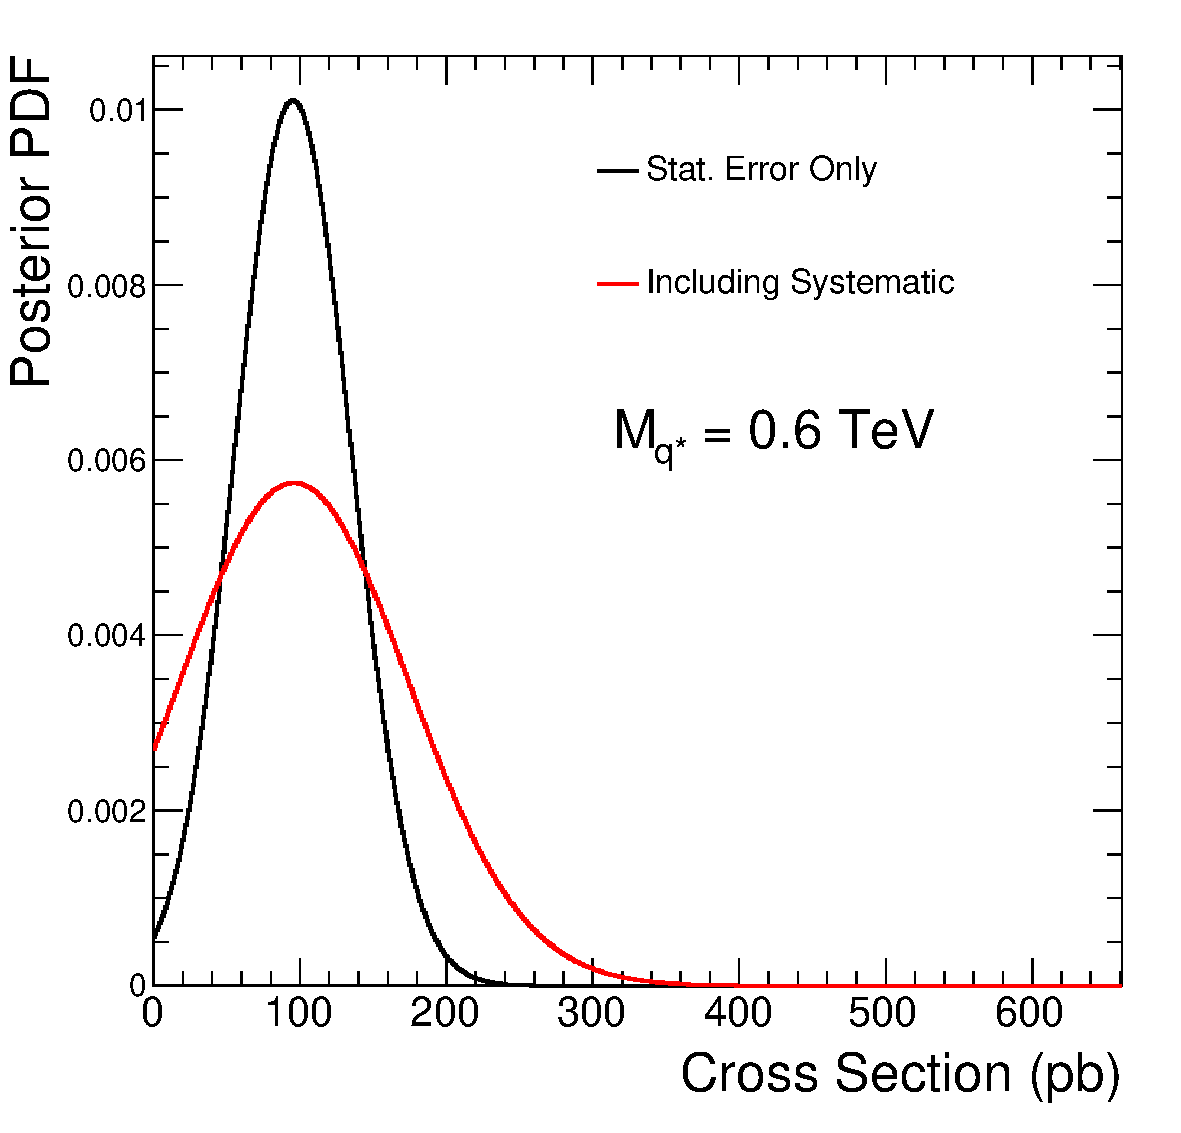
\includegraphics[width=0.48\textwidth]{Figures/Likelihood_600GeV.pdf}
     \includegraphics[width=0.48\textwidth]{Figures/Likelihood_700GeV.pdf}
     \includegraphics[width=0.48\textwidth]{Figures/Likelihood_800GeV.pdf}
 \caption{Posterior probability densities at
 various excited quark resonance masses.  Black histogram includes statistical
 uncertainties only, red histogram includes both statistical and systematic
 uncertainties. The 95\% CL upper limit is the value for which 95\% of 
 the probability corresponds to smaller cross section: the 95\% quantile.}
    \label{likeli}
  \end{center}
\end{figure}

\clearpage

\begin{figure}[!ht]
  \begin{center}
     \includegraphics[width=0.48\textwidth]{Figures/Likelihood_900GeV.pdf}
     \includegraphics[width=0.48\textwidth]{Figures/Likelihood_1000GeV.pdf}
     \includegraphics[width=0.48\textwidth]{Figures/Likelihood_1100GeV.pdf}
     \includegraphics[width=0.48\textwidth]{Figures/Likelihood_1200GeV.pdf}

 \caption{Posterior probability densities at
 various excited quark resonance masses.  Black histogram includes statistical
 uncertainties only, red histogram includes both statistical and systematic
 uncertainties. The 95\% CL upper limit is the value for which 95\% of 
 the probability corresponds to smaller cross section: the 95\% quantile.}
    \label{likeli2}
  \end{center}
\end{figure}

\clearpage

\begin{figure}[!ht]
  \begin{center}
     \includegraphics[width=0.48\textwidth]{Figures/Likelihood_1300GeV.pdf}
     \includegraphics[width=0.48\textwidth]{Figures/Likelihood_1400GeV.pdf}
     \includegraphics[width=0.48\textwidth]{Figures/Likelihood_1500GeV.pdf}
     \includegraphics[width=0.48\textwidth]{Figures/Likelihood_1600GeV.pdf}
 \caption{Posterior probability densities at
 various excited quark resonance masses.  Black histogram includes statistical
 uncertainties only, red histogram includes both statistical and systematic
 uncertainties. The 95\% CL upper limit is the value for which 95\% of 
 the probability corresponds to smaller cross section: the 95\% quantile.}
    \label{likeli3}
  \end{center}
\end{figure}

\clearpage

\begin{figure}[!ht]
  \begin{center}
     \includegraphics[width=0.48\textwidth]{Figures/Likelihood_1700GeV.pdf}
     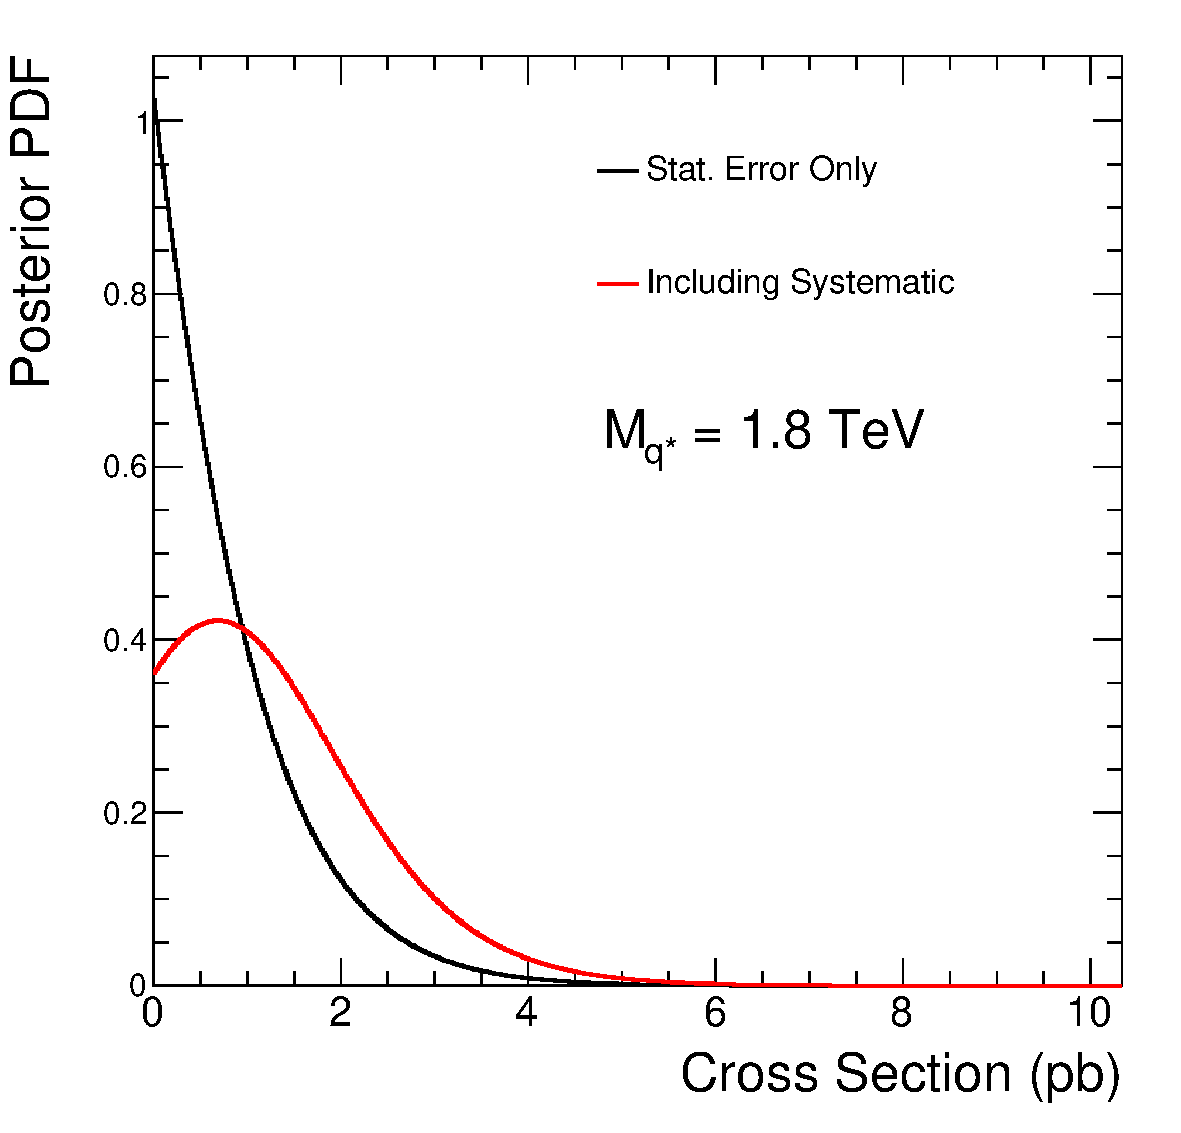
\includegraphics[width=0.48\textwidth]{Figures/Likelihood_1800GeV.pdf}
     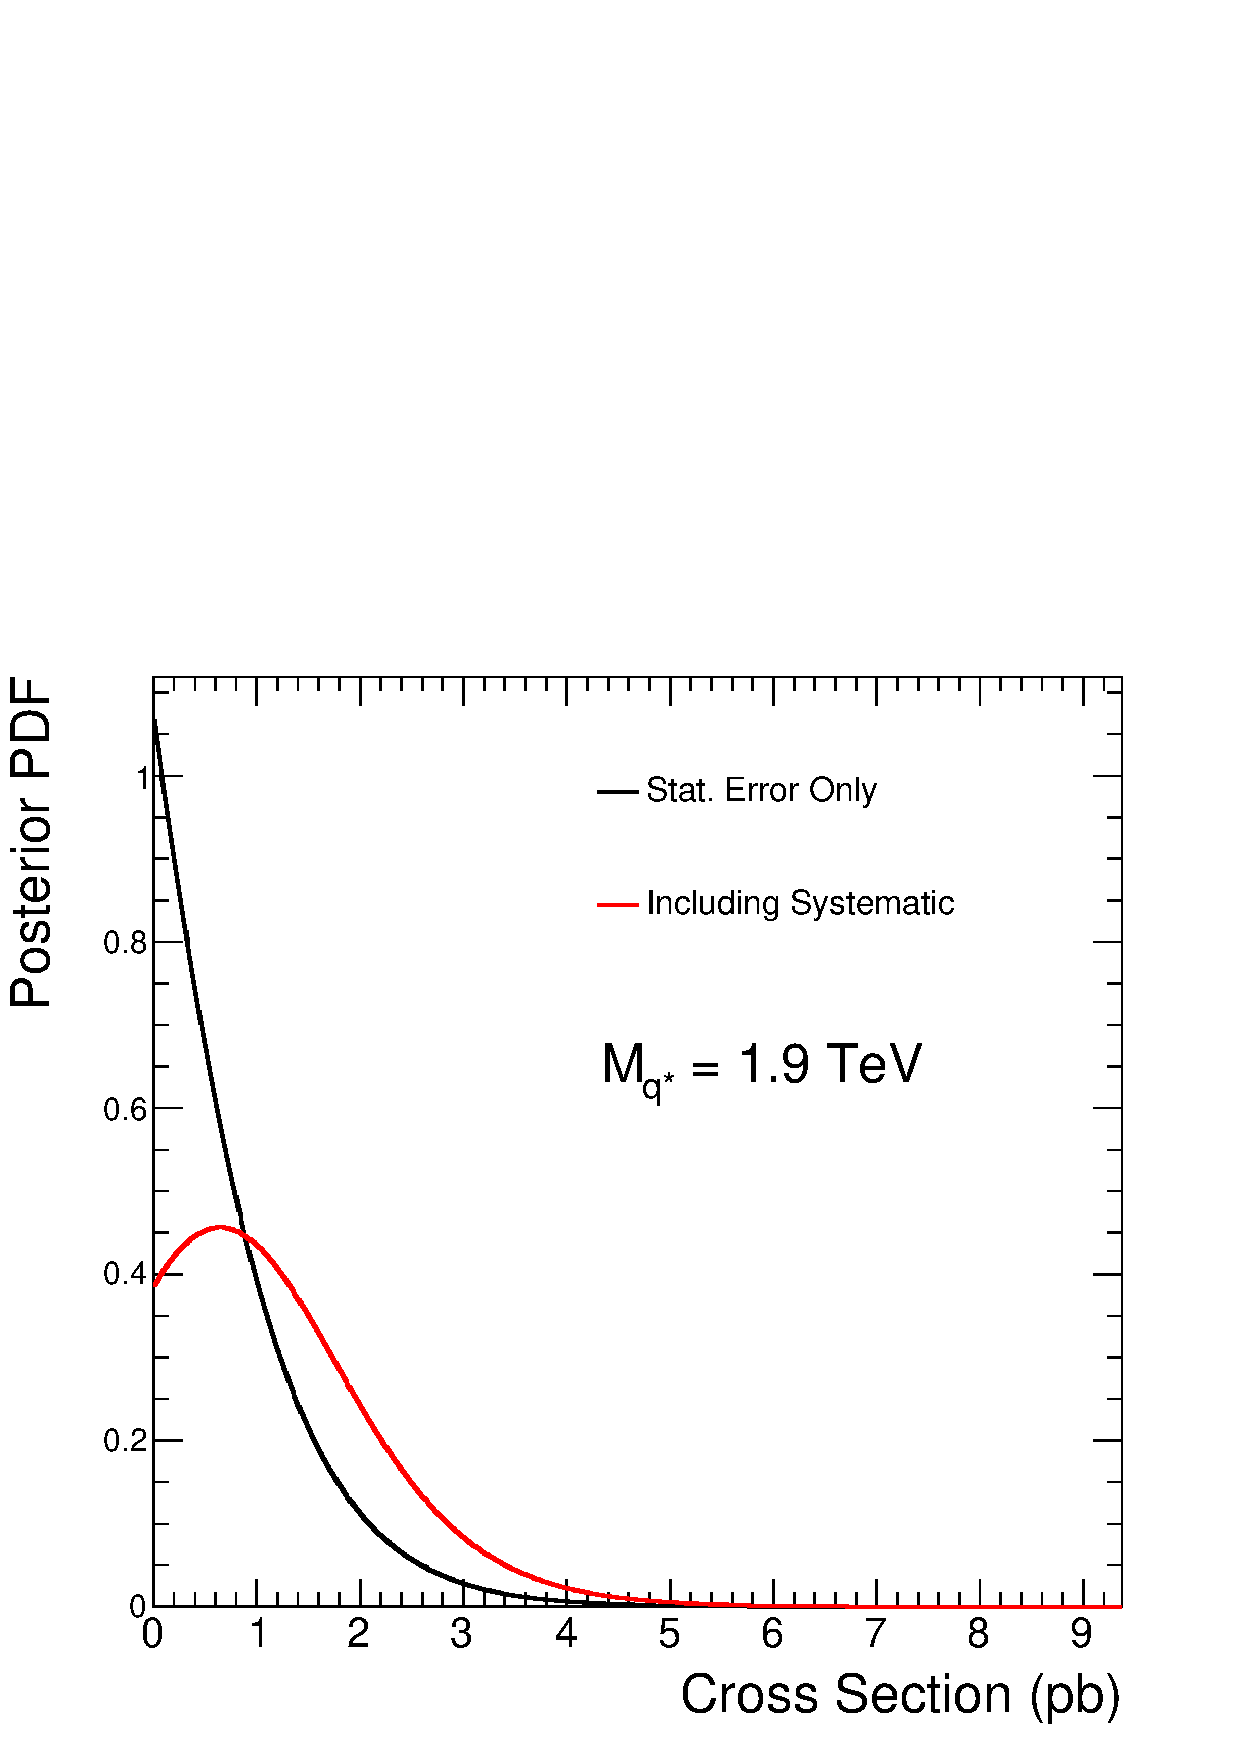
\includegraphics[width=0.48\textwidth]{Figures/Likelihood_1900GeV.pdf}
     \includegraphics[width=0.48\textwidth]{Figures/Likelihood_2000GeV.pdf}
 \caption{Posterior probability densities at
 various excited quark resonance masses.  Black histogram includes statistical
 uncertainties only, red histogram includes both statistical and systematic
 uncertainties. The 95\% CL upper limit is the value for which 95\% of 
 the probability corresponds to smaller cross section: the 95\% quantile.}
    \label{likeli4}
  \end{center}
\end{figure}

\clearpage

\begin{figure}[!ht]
  \begin{center}
     \includegraphics[width=0.48\textwidth]{Figures/Likelihood_2100GeV.pdf}
     \includegraphics[width=0.48\textwidth]{Figures/Likelihood_2200GeV.pdf}
     \includegraphics[width=0.48\textwidth]{Figures/Likelihood_2300GeV.pdf}
     \includegraphics[width=0.48\textwidth]{Figures/Likelihood_2400GeV.pdf}
     \includegraphics[width=0.48\textwidth]{Figures/Likelihood_2500GeV.pdf} 
     \includegraphics[width=0.48\textwidth]{Figures/Likelihood_2600GeV.pdf} 
\caption{Posterior probability densities at
 various excited quark resonance masses.  Black histogram includes statistical
 uncertainties only, red histogram includes both statistical and systematic
 uncertainties. The 95\% CL upper limit is the value for which 95\% of 
 the probability corresponds to smaller cross section: the 95\% quantile.}
    \label{likeli5}
  \end{center}
\end{figure}

